% Day 3: AI Integration with LaTeX
% SUZA Workshop - Scientific Writing with LaTeX & AI
% Compile with: pdflatex

\documentclass[aspectratio=169]{beamer}

% Theme and Color Settings (Classic Academic)
\usetheme{Madrid}
\usecolortheme{default}
\setbeamercolor{structure}{fg=blue!70!black}
\setbeamercolor{frametitle}{bg=blue!10,fg=blue!70!black}
\usefonttheme{serif}

% Packages
\usepackage[utf8]{inputenc}
\usepackage{graphicx}
\usepackage{listings}
\usepackage{xcolor}
\usepackage{hyperref}
\usepackage{amsmath,amssymb}
\usepackage{tikz}

% Code Listing Settings
\lstset{
	basicstyle=\ttfamily\small,
	keywordstyle=\color{blue},
	commentstyle=\color{gray},
	stringstyle=\color{red},
	frame=single,
	breaklines=true,
	numbers=left,
	numberstyle=\tiny\color{gray}
}

% Header and Footer Configuration
\setbeamertemplate{headline}{
	\leavevmode%
	\hbox{%
		\begin{beamercolorbox}[wd=.02\paperwidth,ht=2.5ex,dp=1.125ex]{section in head/foot}%
		\end{beamercolorbox}%
		\begin{beamercolorbox}[wd=.15\paperwidth,ht=2.5ex,dp=1.125ex,left]{section in head/foot}%
			\includegraphics[height=2ex]{../resources/suza_logo.png}
		\end{beamercolorbox}%
		\begin{beamercolorbox}[wd=.81\paperwidth,ht=2.5ex,dp=1.125ex,center]{section in head/foot}%
			\scriptsize State University of Zanzibar (SUZA) | Scientific Writing with LaTeX \& AI
		\end{beamercolorbox}%
	}
	\vskip2pt
	{\color{blue!70!black}\hrule height 0.5pt}
}

\setbeamertemplate{footline}{
	{\color{blue!70!black}\hrule height 0.5pt}
	\vskip2pt
	\leavevmode%
	\hbox{%
		\begin{beamercolorbox}[wd=.5\paperwidth,ht=2.5ex,dp=1.125ex,left,leftskip=1em]{author in head/foot}%
			\scriptsize Masoud Hamad  |  massoud.hamad@suza.ac.tz  |  Department of CS\&IT, SCCMS
		\end{beamercolorbox}%
		\begin{beamercolorbox}[wd=.4\paperwidth,ht=2.5ex,dp=1.125ex,right]{date in head/foot}%
			\scriptsize\insertshortdate
		\end{beamercolorbox}%
		\begin{beamercolorbox}[wd=.1\paperwidth,ht=2.5ex,dp=1.125ex,right,rightskip=1em]{page number in head/foot}%
			\insertframenumber{} / \inserttotalframenumber
		\end{beamercolorbox}
	}%
	\vskip2pt
}

% Title Information
\title{Day 3: AI-Powered Scientific Writing}
\subtitle{Integrating AI Tools with LaTeX for Research Excellence}
\author{Masoud Hamad}
\institute{Department of Computer Science \& Information Technology\\
	School of Computer, Communication and Mathematical Sciences\\
	State University of Zanzibar}
\date{\today}

%==============================================================================
\begin{document}
	
	% Title Slide
	\begin{frame}
		\titlepage
	\end{frame}
	
	% Table of Contents
	\begin{frame}{Today's Agenda}
		\tableofcontents
	\end{frame}
	
	%==============================================================================
	\section{The AI Revolution in Academic Writing}
	
	\begin{frame}{Why AI + LaTeX?}
		\begin{columns}
			\begin{column}{0.48\textwidth}
				\textbf{LaTeX Strengths:}
				\begin{itemize}
					\item Professional typesetting
					\item Mathematical precision
					\item Consistent formatting
					\item Version control friendly
				\end{itemize}
			\end{column}
			
			\begin{column}{0.48\textwidth}
				\textbf{AI Capabilities:}
				\begin{itemize}
					\item Code generation
					\item Content assistance
					\item Language refinement
					\item Research support
				\end{itemize}
			\end{column}
		\end{columns}
		
		\vspace{0.8em}
		
		\begin{exampleblock}{The Synergy}
			Combine LaTeX's precision with AI's efficiency to accelerate high-quality research output while maintaining academic rigor.
		\end{exampleblock}
	\end{frame}
	
	\begin{frame}{Current Landscape of AI Tools}
		\textbf{Large Language Models:}
		\begin{itemize}
			\item ChatGPT (OpenAI) -- General purpose, code generation
			\item Claude (Anthropic) -- Long context, technical writing
			\item Gemini (Google) -- Multimodal, research integration
		\end{itemize}
		
		\vspace{0.5em}
		
		\textbf{Specialized Academic AI:}
		\begin{itemize}
			\item Consensus AI -- Research paper search and synthesis
			\item Semantic Scholar -- AI-powered literature review
			\item Scite -- Citation context and verification
			\item Elicit -- Research question answering
		\end{itemize}
	\end{frame}
	
	\begin{frame}{What AI Can (and Cannot) Do}
		\begin{columns}
			\begin{column}{0.48\textwidth}
				\textbf{AI Excels At:}
				\begin{itemize}
					\item Generating LaTeX code
					\item Formatting assistance
					\item Grammar and style
					\item Literature summaries
					\item Brainstorming ideas
				\end{itemize}
			\end{column}
			
			\begin{column}{0.48\textwidth}
				\textbf{AI Limitations:}
				\begin{itemize}
					\item Cannot verify facts
					\item May hallucinate citations
					\item No true understanding
					\item Requires human oversight
					\item Limited by training data
				\end{itemize}
			\end{column}
		\end{columns}
		
		\vspace{0.8em}
		
		\begin{alertblock}{Critical Principle}
			AI is a powerful assistant, not a replacement for critical thinking and academic integrity.
		\end{alertblock}
	\end{frame}
	
	%==============================================================================
	\section{AI for LaTeX Code Generation}
	
	\begin{frame}{Generating LaTeX with AI Prompts}
		\textbf{Effective Prompting Strategy:}
		\begin{enumerate}
			\item Be specific about document type and requirements
			\item Provide context and examples
			\item Iterate and refine outputs
			\item Verify and customize generated code
		\end{enumerate}
		
		\vspace{0.8em}
		
		\begin{exampleblock}{Example Prompt}
			\small
			"Create a LaTeX table with 3 methods (Baseline, Method A, Method B) and 4 metrics (Accuracy, Precision, Recall, F1). Use booktabs."
		\end{exampleblock}
	\end{frame}
	
	\begin{frame}[fragile]{Example: AI-Generated Table}
		\textbf{Prompt:} "Create a comparison table for ML algorithms"
		
		\vspace{0.3em}
		
		\begin{lstlisting}[language=TeX,basicstyle=\ttfamily\footnotesize]
			\begin{table}[h]
				\centering
				\caption{Algorithm Performance Comparison}
				\begin{tabular}{lccc}
					\toprule
					Algorithm & Accuracy & Time & Memory \\
					\midrule
					Random Forest & 0.94 & 12.3s & 256MB \\
					SVM & 0.91 & 45.7s & 128MB \\
					Neural Net & 0.96 & 180.2s & 512MB \\
					\bottomrule
				\end{tabular}
			\end{table}
		\end{lstlisting}
	\end{frame}
	
	\begin{frame}{Complex Equations Made Easy}
		\textbf{Traditional Approach:}
		\begin{itemize}
			\item Look up syntax for complex symbols
			\item Debug bracket matching
			\item Format multi-line equations
		\end{itemize}
		
		\vspace{0.5em}
		
		\textbf{AI-Assisted Approach:}
		\begin{itemize}
			\item Describe equation in plain language
			\item AI generates LaTeX code
			\item Quick iteration for refinements
		\end{itemize}
		
		\vspace{0.5em}
		
		\begin{block}{Example Prompt}
			"Generate LaTeX for Gaussian PDF with mean mu and variance sigma squared"
		\end{block}
	\end{frame}
	
	\begin{frame}[fragile]{AI-Generated Complex Equation}
		\textbf{Prompt Result:}
		\begin{lstlisting}[language=TeX,basicstyle=\ttfamily\footnotesize]
			\begin{equation}
				f(x|\mu,\sigma^2) = \frac{1}{\sqrt{2\pi\sigma^2}}
				\exp\left(-\frac{(x-\mu)^2}{2\sigma^2}\right)
			\end{equation}
		\end{lstlisting}
		
		\vspace{0.5em}
		
		\textbf{Rendered:}
		\begin{equation}
			f(x|\mu,\sigma^2) = \frac{1}{\sqrt{2\pi\sigma^2}}
			\exp\left(-\frac{(x-\mu)^2}{2\sigma^2}\right)
		\end{equation}
		
		\vspace{0.5em}
		
		\textit{Much faster than manual lookup!}
	\end{frame}
	
	\begin{frame}{Document Structure Templates}
		\textbf{Common AI Template Requests:}
		
		\begin{enumerate}
			\item \textbf{Research Paper:} IEEE conference template with abstract, 5 sections, bibliography
			
			\item \textbf{Thesis Chapter:} Introduction, literature review, methodology, results, discussion
			
			\item \textbf{Lab Report:} Objectives, apparatus, procedure, results, conclusion
			
			\item \textbf{Presentation:} Beamer outline for 20-minute research talk
		\end{enumerate}
		
		\vspace{0.5em}
		
		\textit{AI provides solid starting points to customize!}
	\end{frame}
	
	%==============================================================================
	\section{AI-Powered Research Assistance}
	
	\begin{frame}{Literature Review with AI}
		\begin{columns}[t]
			\begin{column}{0.48\textwidth}
				\textbf{Traditional:}
				\begin{itemize}
					\item Manual searches
					\item Reading abstracts
					\item Organizing findings
					\item Synthesizing
				\end{itemize}
			\end{column}
			
			\begin{column}{0.48\textwidth}
				\textbf{AI-Enhanced:}
				\begin{itemize}
					\item AI summarizes papers
					\item Identifies key themes
					\item Suggests related work
					\item Generates BibTeX
				\end{itemize}
			\end{column}
		\end{columns}
	\end{frame}
	
	\begin{frame}{Tools for Literature Review}
		\begin{description}
			\item[Consensus] Research questions answered from papers
			\item[Semantic Scholar] AI-powered recommendations
			\item[Connected Papers] Visual research landscapes
			\item[Elicit] Automate literature workflows
			\item[Research Rabbit] Citation network discovery
		\end{description}
		
		\vspace{0.5em}
		
		\begin{exampleblock}{Workflow}
			Research tools $\rightarrow$ Export citations $\rightarrow$ AI organize $\rightarrow$ Write in LaTeX
		\end{exampleblock}
	\end{frame}
	
	\begin{frame}[fragile]{Generating BibTeX from AI}
		\textbf{Prompt:} "BibTeX for: 1) Attention is All You Need, 2) AlexNet, 3) BERT"
		
		\vspace{0.3em}
		
		\begin{lstlisting}[language=TeX,basicstyle=\ttfamily\tiny]
			@inproceedings{vaswani2017attention,
				title={Attention is all you need},
				author={Vaswani, Ashish and Shazeer, Noam and others},
				booktitle={NeurIPS},
				year={2017}
			}
			
			@inproceedings{krizhevsky2012imagenet,
				title={Imagenet classification with deep CNNs},
				author={Krizhevsky, Alex and Sutskever, Ilya and Hinton, G.},
				booktitle={NeurIPS},
				year={2012}
			}
		\end{lstlisting}
		
		\begin{alertblock}{Warning}
			\small Always verify AI-generated citations!
		\end{alertblock}
	\end{frame}
	
	\begin{frame}{AI for Data Analysis}
		\textbf{AI Can Help:}
		\begin{itemize}
			\item Interpret statistical significance
			\item Identify patterns and trends
			\item Suggest visualization approaches
			\item Generate LaTeX table formats
			\item Recommend plots (TikZ, PGFPlots)
			\item Draft figure captions
		\end{itemize}
		
		\vspace{0.5em}
		
		\textit{Remember: AI interprets, you validate!}
	\end{frame}
	
	%==============================================================================
	\section{Writing Enhancement with AI}
	
	\begin{frame}{Grammar and Style Refinement}
		\textbf{AI Writing Assistants:}
		\begin{itemize}
			\item Grammarly -- Grammar and clarity
			\item DeepL Write -- Advanced rephrasing
			\item Writefull -- Academic writing specific
			\item QuillBot -- Paraphrasing tool
		\end{itemize}
		
		\vspace{0.5em}
		
		\textbf{Workflow with LaTeX:}
		\begin{enumerate}
			\item Write draft in LaTeX
			\item Export sections to plain text
			\item Process through AI tool
			\item Integrate improvements
		\end{enumerate}
	\end{frame}
	
	\begin{frame}{Improving Academic Tone}
		\begin{exampleblock}{Before (Informal)}
			"The results are really good and show our method works way better."
		\end{exampleblock}
		
		\vspace{0.3em}
		
		\textbf{AI Prompt:} "Rewrite in formal academic tone"
		
		\vspace{0.3em}
		
		\begin{exampleblock}{After (Formal)}
			"The experimental results demonstrate substantial improvements, indicating the proposed method significantly outperforms existing approaches."
		\end{exampleblock}
		
		\vspace{0.5em}
		
		\textbf{AI can also:} Vary sentence structure, suggest stronger vocabulary, eliminate redundancy, improve transitions
	\end{frame}
	
	\begin{frame}{Abstract and Introduction Generation}
		\textbf{Using AI as Starting Point:}
		
		\begin{enumerate}
			\item Provide: Research question, methodology, findings, significance
			\item AI generates draft structure
			\item You refine with: Domain expertise, specific results, citations, guidelines
		\end{enumerate}
		
		\vspace{0.5em}
		
		\begin{alertblock}{Best Practice}
			Never use AI text verbatim. Always revise, verify, and personalize.
		\end{alertblock}
	\end{frame}
	
	\begin{frame}{Paraphrasing for Clarity}
		\textbf{Use Cases:}
		\begin{itemize}
			\item Simplifying complex descriptions
			\item Avoiding repetitive language
			\item Rephrasing awkward sentences
		\end{itemize}
		
		\vspace{0.5em}
		
		\textbf{Workflow:}
		\begin{enumerate}
			\item Identify problematic text
			\item Request alternatives: "Paraphrase maintaining technical accuracy"
			\item Review options and select best
			\item Verify correctness
		\end{enumerate}
		
		\vspace{0.3em}
		
		\begin{block}{Ethical Note}
			Paraphrasing others' work still requires citation.
		\end{block}
	\end{frame}
	
	%==============================================================================
	\section{Practical AI Workflows}
	
	\begin{frame}{Workflow 1: From Idea to Draft}
		\begin{enumerate}
			\item \textbf{Brainstorm:} Explore research angles with AI
			\item \textbf{Structure:} Generate LaTeX skeleton
			\item \textbf{Literature:} AI identifies relevant papers
			\item \textbf{Method:} Draft methodology with AI
			\item \textbf{Results:} AI suggests formats
			\item \textbf{Writing:} Compose with AI support
			\item \textbf{References:} Generate BibTeX entries
			\item \textbf{Polish:} AI refines clarity
		\end{enumerate}
		
		\vspace{0.5em}
		
		\textit{Humans drive; AI accelerates.}
	\end{frame}
	
	\begin{frame}{Workflow 2: Notes to Paper}
		\textbf{Scenario:} Transform research notes into formatted paper
		
		\vspace{0.5em}
		
		\textbf{Process:}
		\begin{enumerate}
			\item Share organized notes with AI
			\item AI suggests paper structure
			\item Generate LaTeX template
			\item AI expands notes into prose
			\item Add technical details and proofs
			\item AI formats equations and tables
			\item Final human review
		\end{enumerate}
		
		\vspace{0.5em}
		
		\textbf{Time savings:} 40-60\% reduction in drafting time
	\end{frame}
	
	\begin{frame}{Workflow 3: Debugging LaTeX}
		\textbf{When Compilation Fails:}
		
		\begin{enumerate}
			\item Copy error message
			\item Ask AI: "Fix this LaTeX error: [paste]"
			\item AI explains the problem
			\item AI suggests correction
			\item Implement and test
		\end{enumerate}
		
		\vspace{0.5em}
		
		\begin{exampleblock}{Example}
			\textbf{Error:} "Missing \$ inserted"
			
			\textbf{AI:} "Math symbols (\_) need math mode. Use \$x\_i\$ or x\textbackslash\_i"
		\end{exampleblock}
		
		\vspace{0.3em}
		
		\textit{AI excels at explaining errors!}
	\end{frame}
	
	\begin{frame}[fragile]{Workflow 4: Creating Diagrams}
		\textbf{TikZ Code Generation:}
		
		Prompt: "TikZ neural network: 3 inputs, 2 hidden layers (4 nodes), 2 outputs"
		
		\vspace{0.3em}
		
		\begin{lstlisting}[language=TeX,basicstyle=\ttfamily\tiny]
			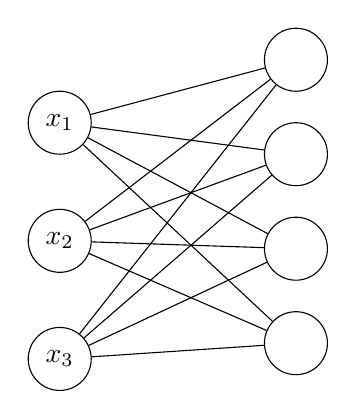
\begin{tikzpicture}[
				neuron/.style={circle,draw,minimum size=0.8cm}]
				
				% Input layer
				\foreach \i in {1,2,3}
				\node[neuron] (I\i) at (0,-\i*1.5) {$x_\i$};
				
				% Hidden layer 1
				\foreach \i in {1,...,4}
				\node[neuron] (H1\i) at (3,-\i*1.2+0.5) {};
				
				% Connections
				\foreach \i in {1,2,3}
				\foreach \j in {1,...,4}
				\draw (I\i) -- (H1\j);
			\end{tikzpicture}
		\end{lstlisting}
	\end{frame}
	
	%==============================================================================
	\section{Ethics and Best Practices}
	
	\begin{frame}{Academic Integrity}
		\begin{alertblock}{Critical Principles}
			\begin{itemize}
				\item AI is a \textbf{tool}, not an author
				\item Always verify facts and citations
				\item Original thinking must be yours
				\item Disclose AI usage when required
			\end{itemize}
		\end{alertblock}
		
		\vspace{0.5em}
		
		\begin{columns}[t]
			\begin{column}{0.48\textwidth}
				\textbf{Acceptable:}
				\begin{itemize}
					\item Code generation
					\item Grammar improvement
					\item Brainstorming
				\end{itemize}
			\end{column}
			
			\begin{column}{0.48\textwidth}
				\textbf{Unacceptable:}
				\begin{itemize}
					\item AI work as your own
					\item Fabricating citations
					\item Bypassing learning
				\end{itemize}
			\end{column}
		\end{columns}
	\end{frame}
	
	\begin{frame}{Verification Checklist}
		\textbf{Before Using AI Content:}
		
		\begin{enumerate}
			\item \textbf{Citations:} Verify references exist and are accurate
			\item \textbf{Facts:} Cross-check with authoritative sources
			\item \textbf{Code:} Test LaTeX compiles correctly
			\item \textbf{Logic:} Ensure arguments are sound
			\item \textbf{Originality:} Check for plagiarism
			\item \textbf{Guidelines:} Follow institutional policies
		\end{enumerate}
		
		\vspace{0.5em}
		
		\begin{block}{Remember}
			You are responsible for everything in your submission.
		\end{block}
	\end{frame}
	
	\begin{frame}{Institutional Policies}
		\textbf{Know Your Rules:}
		\begin{itemize}
			\item Institutions have different AI policies
			\item Some require disclosure
			\item Funding agencies may have restrictions
			\item Journal guidelines vary
		\end{itemize}
		
		\vspace{0.5em}
		
		\textbf{SUZA Guidelines:}
		\begin{itemize}
			\item Consult your supervisor
			\item Check department policies
			\item Document AI usage
			\item Maintain academic honesty
		\end{itemize}
		
		\vspace{0.5em}
		
		\textit{When in doubt, ask!}
	\end{frame}
	
	\begin{frame}{Transparency and Attribution}
		\textbf{Consider Acknowledging AI:}
		
		\begin{itemize}
			\item Methods: "AI tools assisted with code generation"
			\item Acknowledgments: "ChatGPT/Claude aided formatting"
			\item Supplementary: Document AI interactions
		\end{itemize}
		
		\vspace{0.5em}
		
		\textbf{Document:} Which tools, for what purposes, extent of use, verification steps
		
		\vspace{0.5em}
		
		\begin{exampleblock}{Sample}
			"The author used Claude AI to assist with LaTeX formatting. All content independently verified."
		\end{exampleblock}
	\end{frame}
	
	\begin{frame}{Future of AI in Academia}
		\textbf{Emerging Trends:}
		\begin{itemize}
			\item AI integrated into LaTeX editors
			\item Automated peer review assistance
			\item Real-time collaboration with AI
			\item Multimodal research assistants
		\end{itemize}
		
		\vspace{0.5em}
		
		\textbf{Skills for the Future:}
		\begin{itemize}
			\item Prompt engineering
			\item Critical evaluation of AI output
			\item Ethical AI use
			\item Combining human and AI strengths
		\end{itemize}
		
		\vspace{0.3em}
		
		\textit{Goal: Augment intelligence, not replace it.}
	\end{frame}
	
	%==============================================================================
	\section{Hands-On Final Project}
	
	\begin{frame}{Final Project Overview}
		\textbf{Create a Complete Research Document:}
		
		\begin{itemize}
			\item Choose your research topic
			\item Use LaTeX for preparation
			\item Integrate AI throughout
			\item Produce 4-6 page professional paper
		\end{itemize}
		
		\vspace{0.5em}
		
		\textbf{Required Components:}
		\begin{itemize}
			\item Title, abstract, keywords
			\item Introduction with literature review
			\item Methodology section
			\item At least 2 figures/tables, 5 references (BibTeX)
			\item Proper formatting and citations
		\end{itemize}
	\end{frame}
	
	\begin{frame}{Project Guidelines}
		\textbf{AI Usage (minimum 3 tasks):}
		\begin{itemize}
			\item LaTeX code generation
			\item Content outlining/brainstorming
			\item Grammar/style improvement
			\item Bibliography management
			\item Table/figure creation
		\end{itemize}
		
		\vspace{0.5em}
		
		\textbf{Deliverables:}
		\begin{enumerate}
			\item Compiled PDF document
			\item Source .tex files
			\item references.bib file
			\item Brief reflection on AI usage (1 paragraph)
		\end{enumerate}
	\end{frame}
	
	\begin{frame}{Suggested Topics}
		\begin{itemize}
			\item Impact of technology on education in Zanzibar
			\item Climate change effects on coastal communities
			\item Machine learning in healthcare
			\item Cybersecurity in developing nations
			\item Sustainable tourism development
			\item Mobile technology for agriculture
			\item Data science in public health
			\item Any topic in your field of study
		\end{itemize}
		
		\vspace{0.5em}
		
		\textit{Choose something genuinely interesting!}
	\end{frame}
	
	\begin{frame}{Project Workflow}
		\begin{enumerate}
			\item \textbf{Topic (5 min):} Choose and refine
			\item \textbf{Planning (10 min):} AI creates outline
			\item \textbf{Template (10 min):} Generate LaTeX
			\item \textbf{Literature (20 min):} Find 5-10 refs, BibTeX
			\item \textbf{Writing (40 min):} Draft with AI
			\item \textbf{Visuals (15 min):} Create tables/figures
			\item \textbf{Refinement (20 min):} Polish
			\item \textbf{Compilation (10 min):} Debug and finalize
		\end{enumerate}
		
		\vspace{0.3em}
		
		\textbf{Total: ~2 hours}
	\end{frame}
	
	\begin{frame}{AI Prompts to Get Started}
		\begin{enumerate}
			\item "LaTeX article template for [topic] with abstract, intro, methods, results, discussion, references"
			
			\item "Outline for paper on [topic] with key points per section"
			
			\item "BibTeX entry for [paper title/author]"
			
			\item "LaTeX table comparing [items] across [metrics]"
			
			\item "Improve academic tone: [your text]"
			
			\item "Fix LaTeX error: [error message]"
		\end{enumerate}
	\end{frame}
	
	\begin{frame}{Working Session}
		\begin{block}{Next 2 Hours: Project Time}
			\begin{itemize}
				\item Work individually or in pairs
				\item Instructors available for help
				\item Use all Days 1-3 resources
				\item Leverage AI wisely
				\item Ask questions!
			\end{itemize}
		\end{block}
		
		\vspace{0.5em}
		
		\textbf{Checkpoints:}
		\begin{itemize}
			\item 30 min: Topic and outline
			\item 60 min: Draft structure
			\item 90 min: Content and visuals
			\item 120 min: Final document
		\end{itemize}
	\end{frame}
	
	%==============================================================================
	\section{Resources and Next Steps}
	
	\begin{frame}{AI Tools Summary}
		\begin{description}
			\item[General AI:] ChatGPT, Claude, Gemini
			\item[LaTeX:] Overleaf AI, LaTeX prompts
			\item[Research:] Consensus, Semantic Scholar, Elicit
			\item[Writing:] Grammarly, DeepL Write, Writefull
			\item[Citations:] Zotero, Mendeley
			\item[Diagrams:] QuickLatex, Mathpix
		\end{description}
		
		\vspace{0.5em}
		
		\textbf{Free tiers available for most tools}
	\end{frame}
	
	\begin{frame}{Continuing Your Learning}
		\textbf{Practice Projects:}
		\begin{itemize}
			\item Convert old documents to LaTeX
			\item Create presentation templates
			\item Build personal template library
		\end{itemize}
		
		\vspace{0.5em}
		
		\textbf{Communities:}
		\begin{itemize}
			\item TeX Stack Exchange
			\item r/LaTeX on Reddit
			\item Overleaf webinars
		\end{itemize}
		
		\vspace{0.5em}
		
		\textbf{Stay Updated:} AI tools evolve rapidly
	\end{frame}
	
	\begin{frame}{Workshop Resources}
		\textbf{Included Materials:}
		
		\begin{itemize}
			\item All three days' presentations
			\item Sample templates (article, report, thesis)
			\item Practice exercises with solutions
			\item AI prompts reference guide
			\item LaTeX cheat sheet
			\item BibTeX examples
			\item TikZ diagram samples
		\end{itemize}
		
		\vspace{0.5em}
		
		\textbf{Access:} Workshop repository, Overleaf, SUZA platform
	\end{frame}
	
	\begin{frame}{Final Thoughts}
		\begin{block}{Key Takeaways}
			\begin{enumerate}
				\item LaTeX provides professional typesetting
				\item AI accelerates the writing process
				\item Critical thinking remains essential
				\item Combining both creates powerful workflows
				\item Academic integrity is paramount
			\end{enumerate}
		\end{block}
		
		\vspace{0.5em}
		
		\textbf{Moving Forward:} Start simple, incorporate AI gradually, build templates, share knowledge, keep learning
	\end{frame}
	
	\begin{frame}{Feedback and Certification}
		\textbf{Workshop Feedback:}
		\begin{itemize}
			\item Complete the evaluation form
			\item Help improve future workshops
			\item Suggest advanced topics
		\end{itemize}
		
		\vspace{0.5em}
		
		\textbf{Certificate:}
		\begin{itemize}
			\item Submit your final project
			\item Certificates issued within one week
			\item Professional development record
		\end{itemize}
		
		\vspace{0.5em}
		
		\textbf{Stay Connected:} SUZA LaTeX user group, monthly meetups
	\end{frame}
	
	%==============================================================================
	\begin{frame}[plain]
		\centering
		\vspace{2em}
		
		{\Huge\textbf{Thank You!}}
		
		\vspace{2em}
		
		{\large Workshop Complete!}
		
		\vspace{2em}
		
		{\normalsize Questions? Let's discuss!}
		
		\vspace{2em}
		
		Masoud Hamad\\
		massoud.hamad@suza.ac.tz\\
		Department of CS\&IT, SCCMS
		
		\vspace{2em}
		
		{\small Keep creating excellent research!}
	\end{frame}
	
\end{document}